\subsection{Ca sử dụng đăng nhập}
\vspace{0.5cm}

\noindent 
\begin{tabularx}{\linewidth}{| l | X |} 
\hline 
\textbf{Mô tả} & Khi người dùng muốn sử dụng các chức năng yêu cầu quyền đăng nhập. \\ 
\hline 
\textbf{Luồng cơ bản} & 1. Truy cập trang đăng nhập \newline 
                      2. Nhập thông tin tài khoản (email / mật khẩu) \newline 
                      3. Điều hướng đến trang home - danh sách chuyến đi công khai. \\ 
\hline 
\textbf{Luồng thay thế} & - Nếu Người dùng nhập sai thông tin tài khoản hệ thống sẽ thông báo lỗi trên form đăng nhập  \newline 
                       - Người dùng có tài khoản chưa có thông tin sở thích hệ thống điều hướng đến trang khảo sát sở thích \\
\hline 
\textbf{Tiền điều kiện} & Người dùng đã đăng xuất. \\ 
\hline 
\textbf{Hậu điều kiện} & Hệ thống lưu token đăng nhập vào local trên thiết bị. \\ 
\hline 
\textbf{Yêu cầu phi chức năng} & Hệ thống xử lý đăng nhập không quá 2s. \\ 
\hline 
\end{tabularx}

\vspace{0.8cm}

\noindent 
\begin{tabular}{| c | c |}
    \hline
    \textbf{Biểu đồ hoạt động} & \textbf{Quan hệ} \\ 
    \hline
    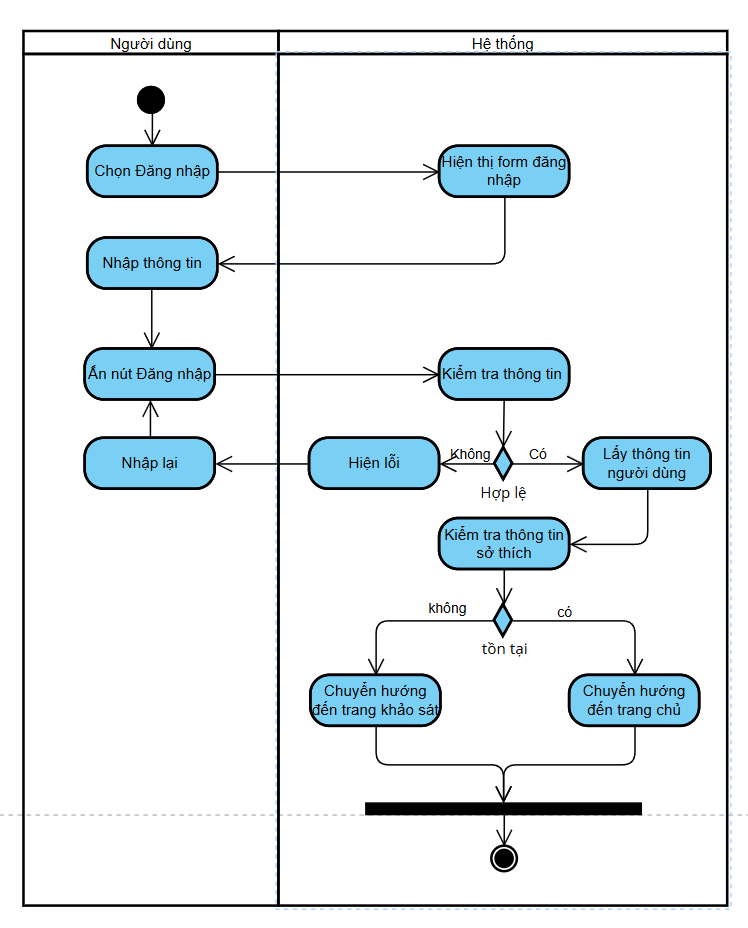
\includegraphics[width=0.5\linewidth]{figures/c3/3-3-2-ad.png} 
    & 
    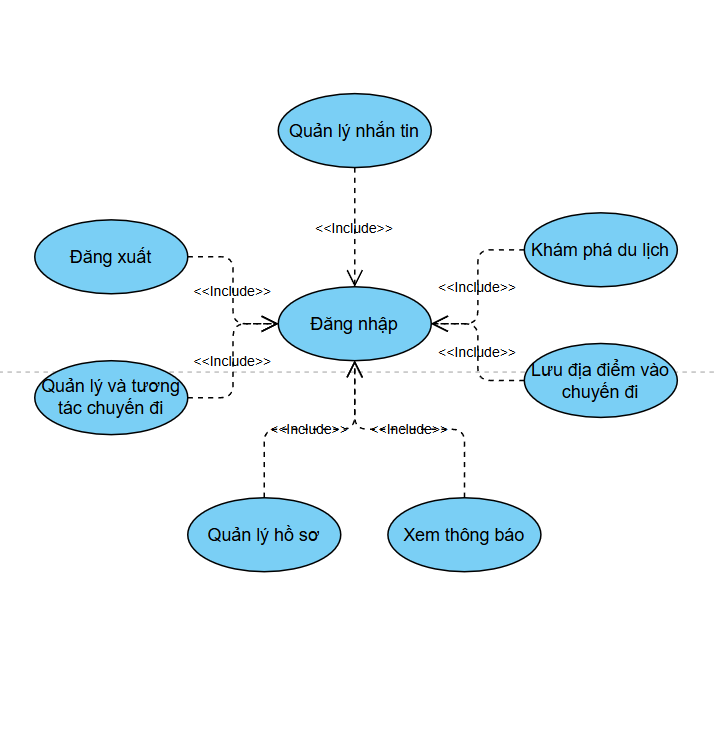
\includegraphics[width=0.45\linewidth]{figures/c3/3-3-2-rd.png} \\ 
    \hline
\end{tabular}
\vspace{0.8cm}

\begin{figure}[H]
    \centering  
    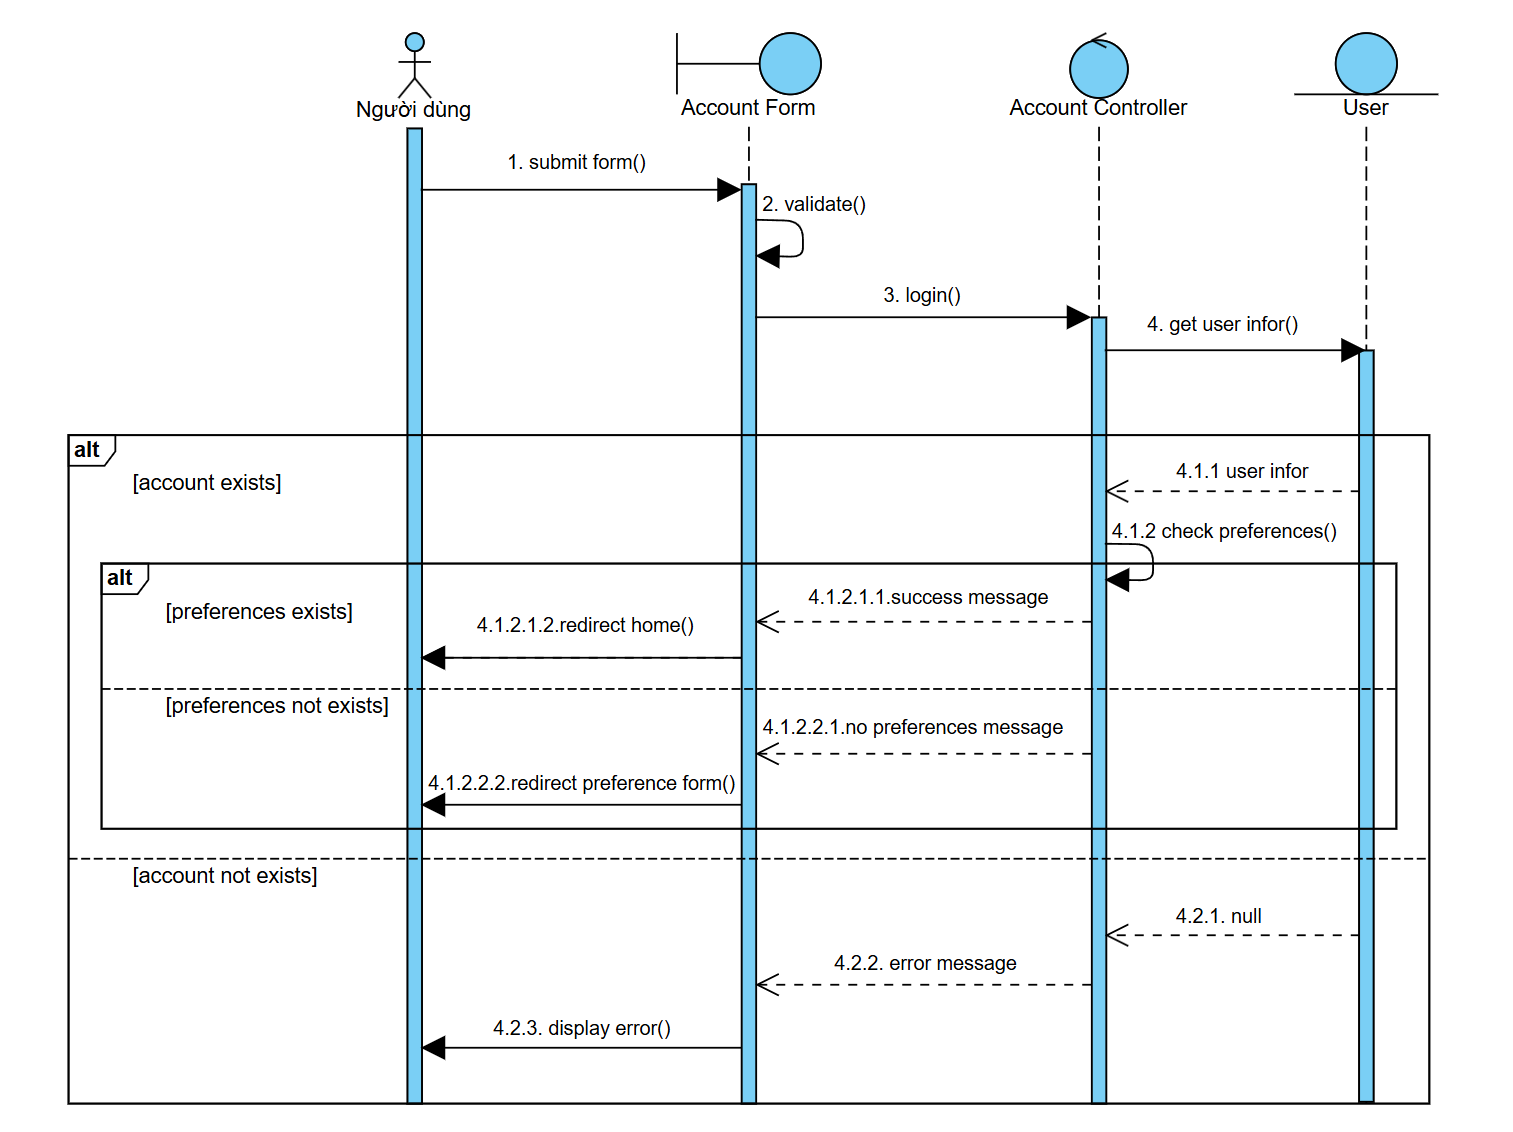
\includegraphics[width=1.05\textwidth]{figures/c3/3-3-2-sd.png}
    \caption{Biểu đồ tuần tự ca sử dụng đăng nhập.}
    \label{fig:3-3-1-sequence-diagram}
\end{figure}